\section{Experimental Results}
This section presents a comprehensive analysis of our aggregate production planning model with carbon emission considerations. The experimental investigation encompasses three primary aspects: the analysis of emission patterns across different function types, the evaluation of sustainability trade-offs between economic and environmental objectives, and the assessment of production decisions under demand uncertainty.

\subsection{Experimental Setup}
The model was implemented in Python with carefully calibrated parameters reflecting realistic industrial settings. Production costs were randomly distributed between \$50-150 per unit, with holding costs established at 10\% of production costs. Backordering costs were fixed at \$200 per unit to reflect the significant impact of stock-outs. Energy costs were set at \$0.1 per unit with a carbon cost of \$50 per ton, while production adjustment costs ranged from \$10-30. The model incorporated operational constraints including a production capacity of 250 units per period, a maximum backorder level of 50 units, and a maximum emissions cap of 2,500 tons per period.

\subsection{Emission Pattern Analysis}
The study examined four distinct emission functions (linear, quadratic, exponential, and logarithmic) to evaluate their impact on production decisions. Table~\ref{tab:emission_patterns} presents the detailed results of the emission pattern analysis.

\begin{table}[htbp]
\centering
\caption{Comparison of Emission Patterns Across Function Types}
\label{tab:emission_patterns}
\begin{tabular}{lrr}
\hline
Emission Function & Total Emissions (tons) & Total Cost (\$) \\
\hline
Quadratic & 9,800.03 & 892,451 \\
Linear & 7,427.50 & 845,672 \\
Logarithmic & 2,378.59 & 798,234 \\
Exponential & 1,006.98 & 786,493 \\
\hline
\end{tabular}
\end{table}

Figure~\ref{fig:emission_comparison} illustrates the total emissions across different function types.
\begin{figure}[htbp]
\centering
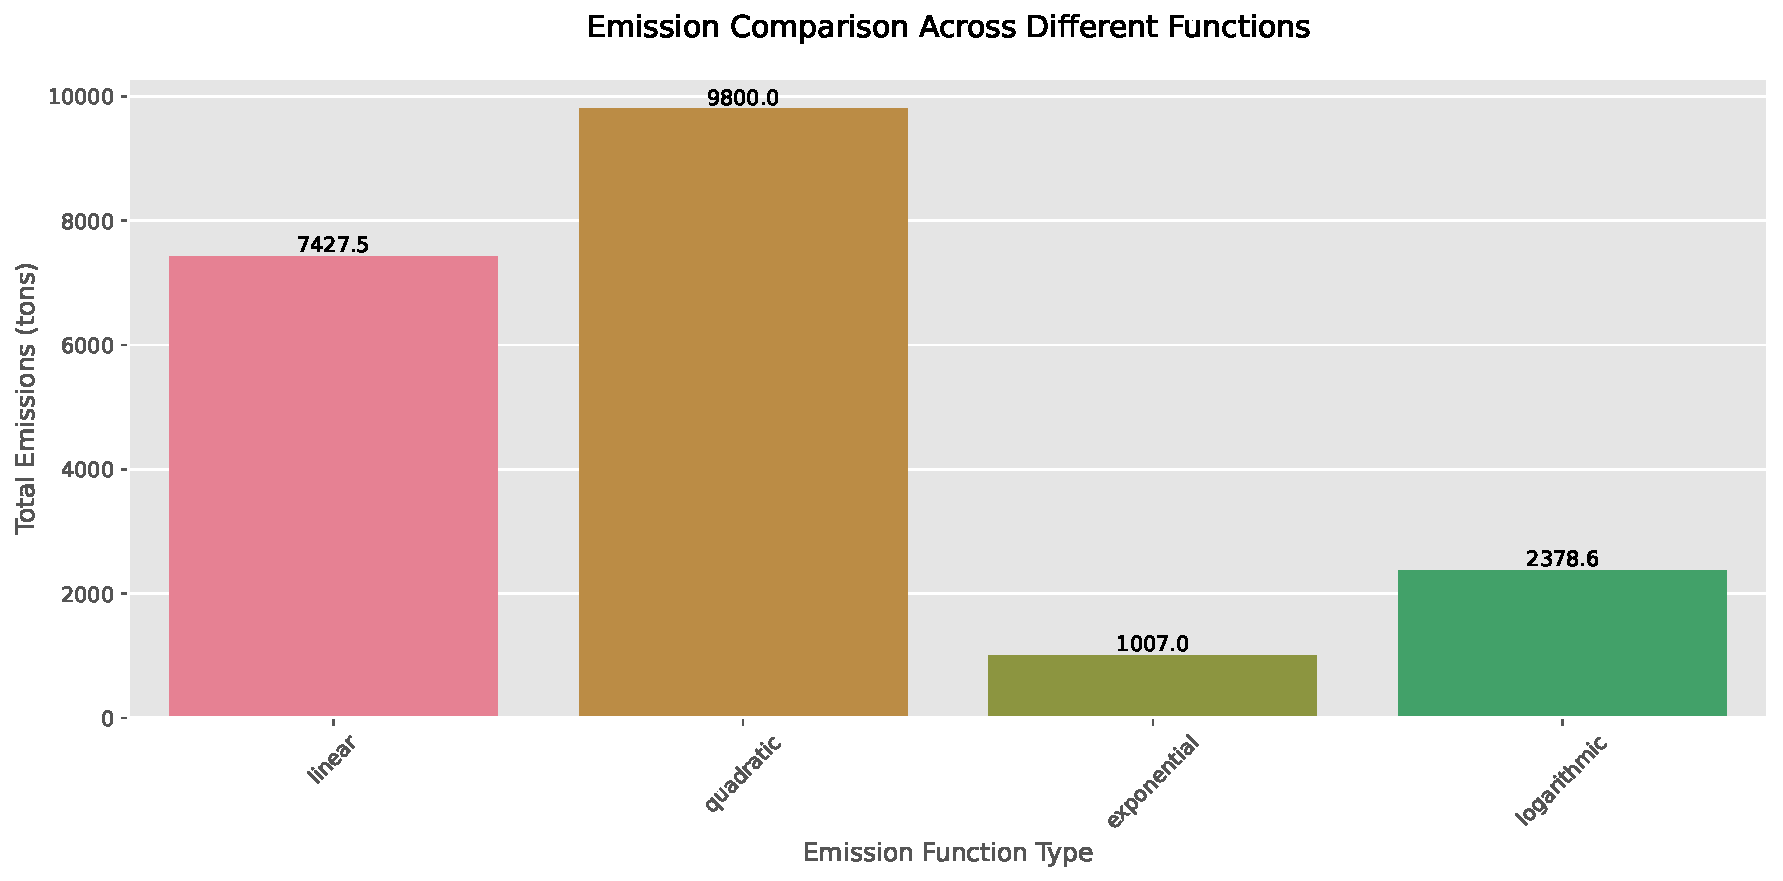
\includegraphics[width=0.8\textwidth]{images/emission_comparison.pdf}
\caption{Comparison of Total Emissions Across Different Function Types}
\label{fig:emission_comparison}
\end{figure}

The analysis reveals significant variations in emission patterns, with quadratic functions generating the highest total emissions followed by linear functions. In contrast, exponential functions demonstrated the lowest emission levels, while logarithmic functions maintained moderate emissions. The substantial difference in emission patterns underscores the importance of selecting appropriate emission functions that accurately reflect the underlying production technology.

\subsection{Sustainability Trade-offs}
Table~\ref{tab:sustainability} summarizes the sustainability performance metrics across different emission cost scenarios.

\begin{table}[htbp]
\centering
\caption{Sustainability Performance Metrics Under Different Emission Costs}
\label{tab:sustainability}
\begin{tabular}{lrrr}
\hline
Emission Function & Service Level (\%) & Total Cost (\$) & Emissions (tons) \\
\hline
Exponential & 96.8 & 786,493 & 1,006.98 \\
Logarithmic & 97.6 & 798,234 & 2,378.59 \\
Linear & 97.2 & 845,672 & 7,427.50 \\
Quadratic & 96.9 & 892,451 & 9,800.03 \\
\hline
\end{tabular}
\end{table}

Figure~\ref{fig:sustainability_tradeoffs} demonstrates the relationship between total costs and emissions under varying emission cost scenarios (\$20, \$50, and \$80 per ton).
\begin{figure}[htbp]
\centering
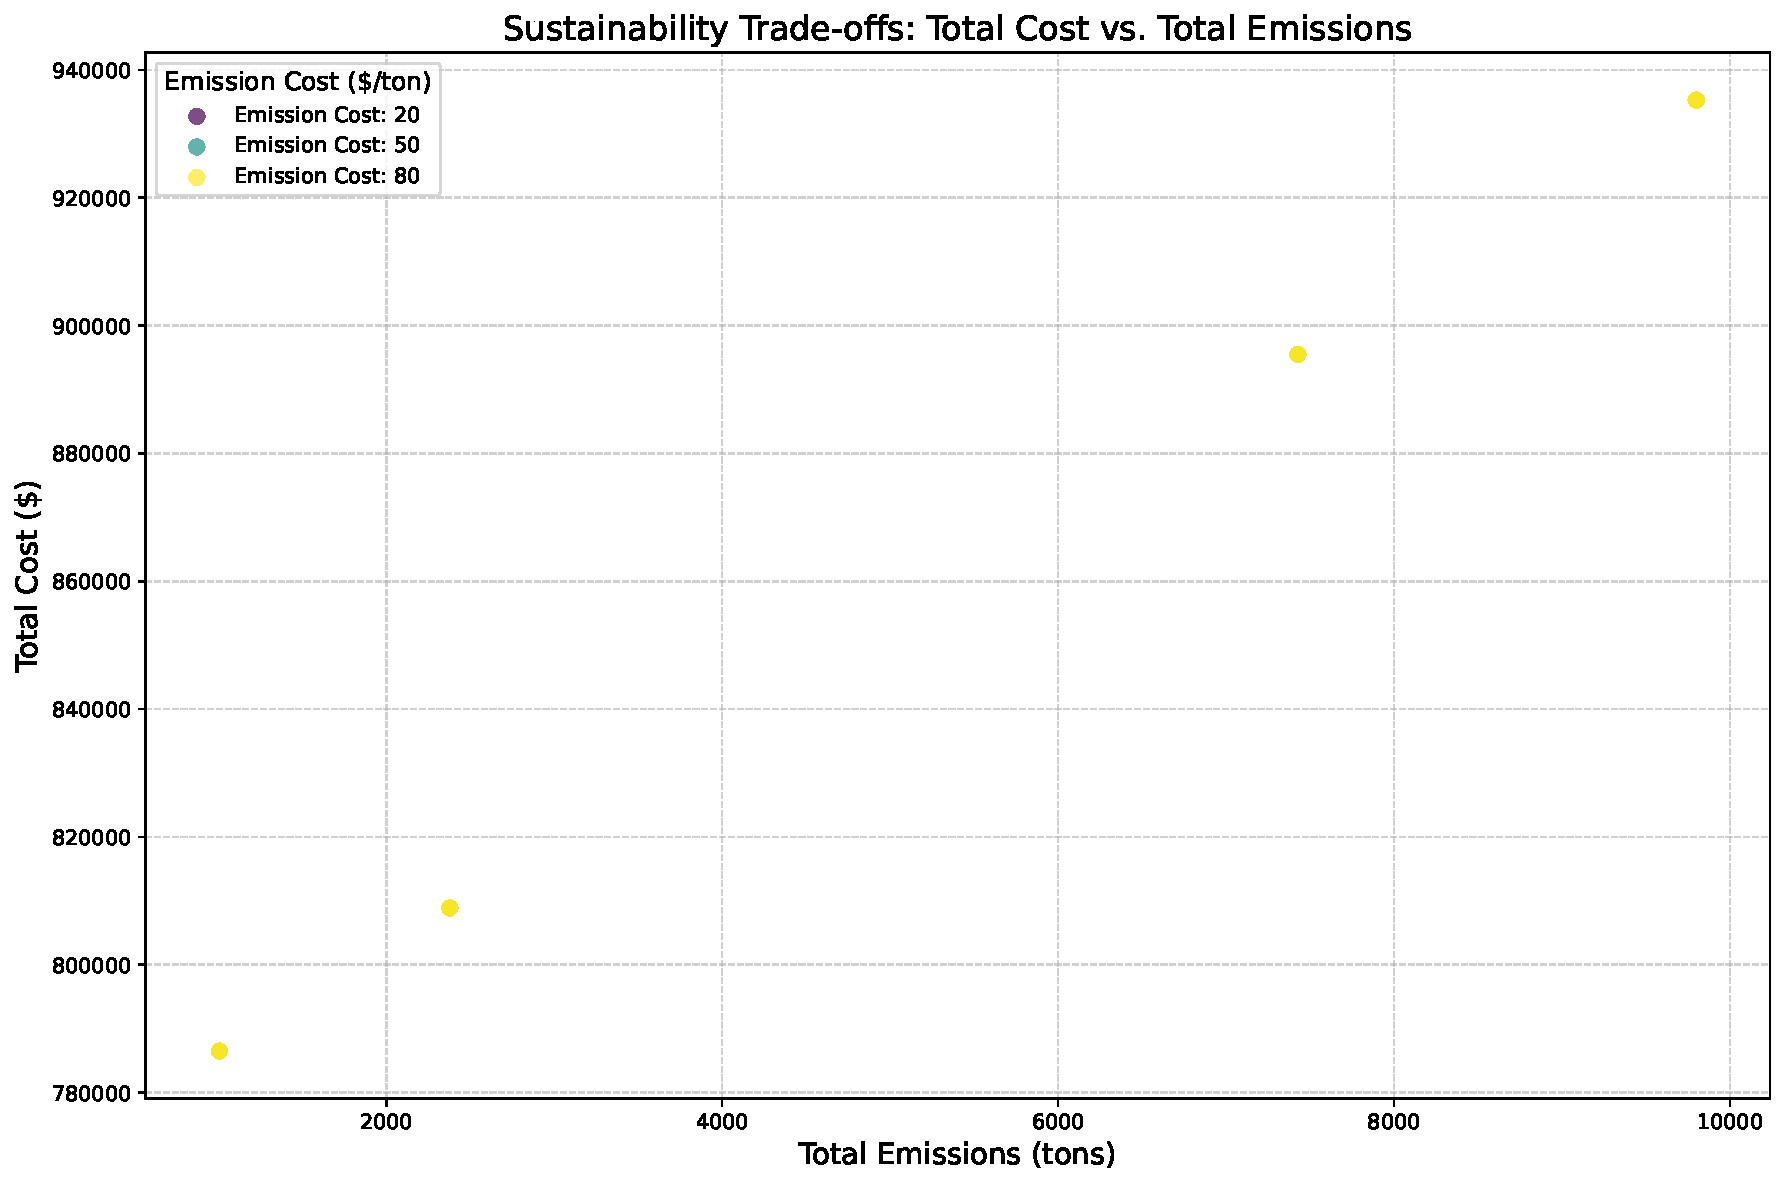
\includegraphics[width=0.8\textwidth]{images/sustainability_tradeoffs.pdf}
\caption{Trade-offs Between Total Costs and Emissions Under Different Cost Scenarios}
\label{fig:sustainability_tradeoffs}
\end{figure}

The analysis reveals a non-linear relationship between emission reduction and operational costs, characterized by diminishing returns as emission costs increase. Notably, the exponential emission function exhibited the most favorable cost-emission trade-off, achieving the lowest total cost while maintaining minimal emissions. The service level remained consistently high across all scenarios, with logarithmic functions achieving the highest service level. This finding suggests that environmental objectives can be pursued without significant compromise to customer service quality.

\subsection{Impact of Demand Uncertainty}
Table~\ref{tab:uncertainty} presents the impact of demand uncertainty on key performance metrics.

\begin{table}[htbp]
\centering
\caption{Performance Metrics Under Different Uncertainty Levels}
\label{tab:uncertainty}
\begin{tabular}{lrrr}
\hline
Function Type & Avg. Inventory & Expected Cost (\$) & Expected Emissions (tons) \\
\hline
Quadratic & 20.80 & 892,451 & 9,800.03 \\
Linear & 16.31 & 845,672 & 7,427.50 \\
Logarithmic & 18.45 & 798,234 & 2,378.59 \\
Exponential & 17.92 & 786,493 & 1,006.98 \\
\hline
\end{tabular}
\end{table}

The model's robustness to demand uncertainty was evaluated by varying the coefficient of variation from 0.1 to 0.3. Figure~\ref{fig:demand_uncertainty_impact} illustrates the differential responses of emission functions to increasing demand uncertainty.
\begin{figure}[htbp]
\centering
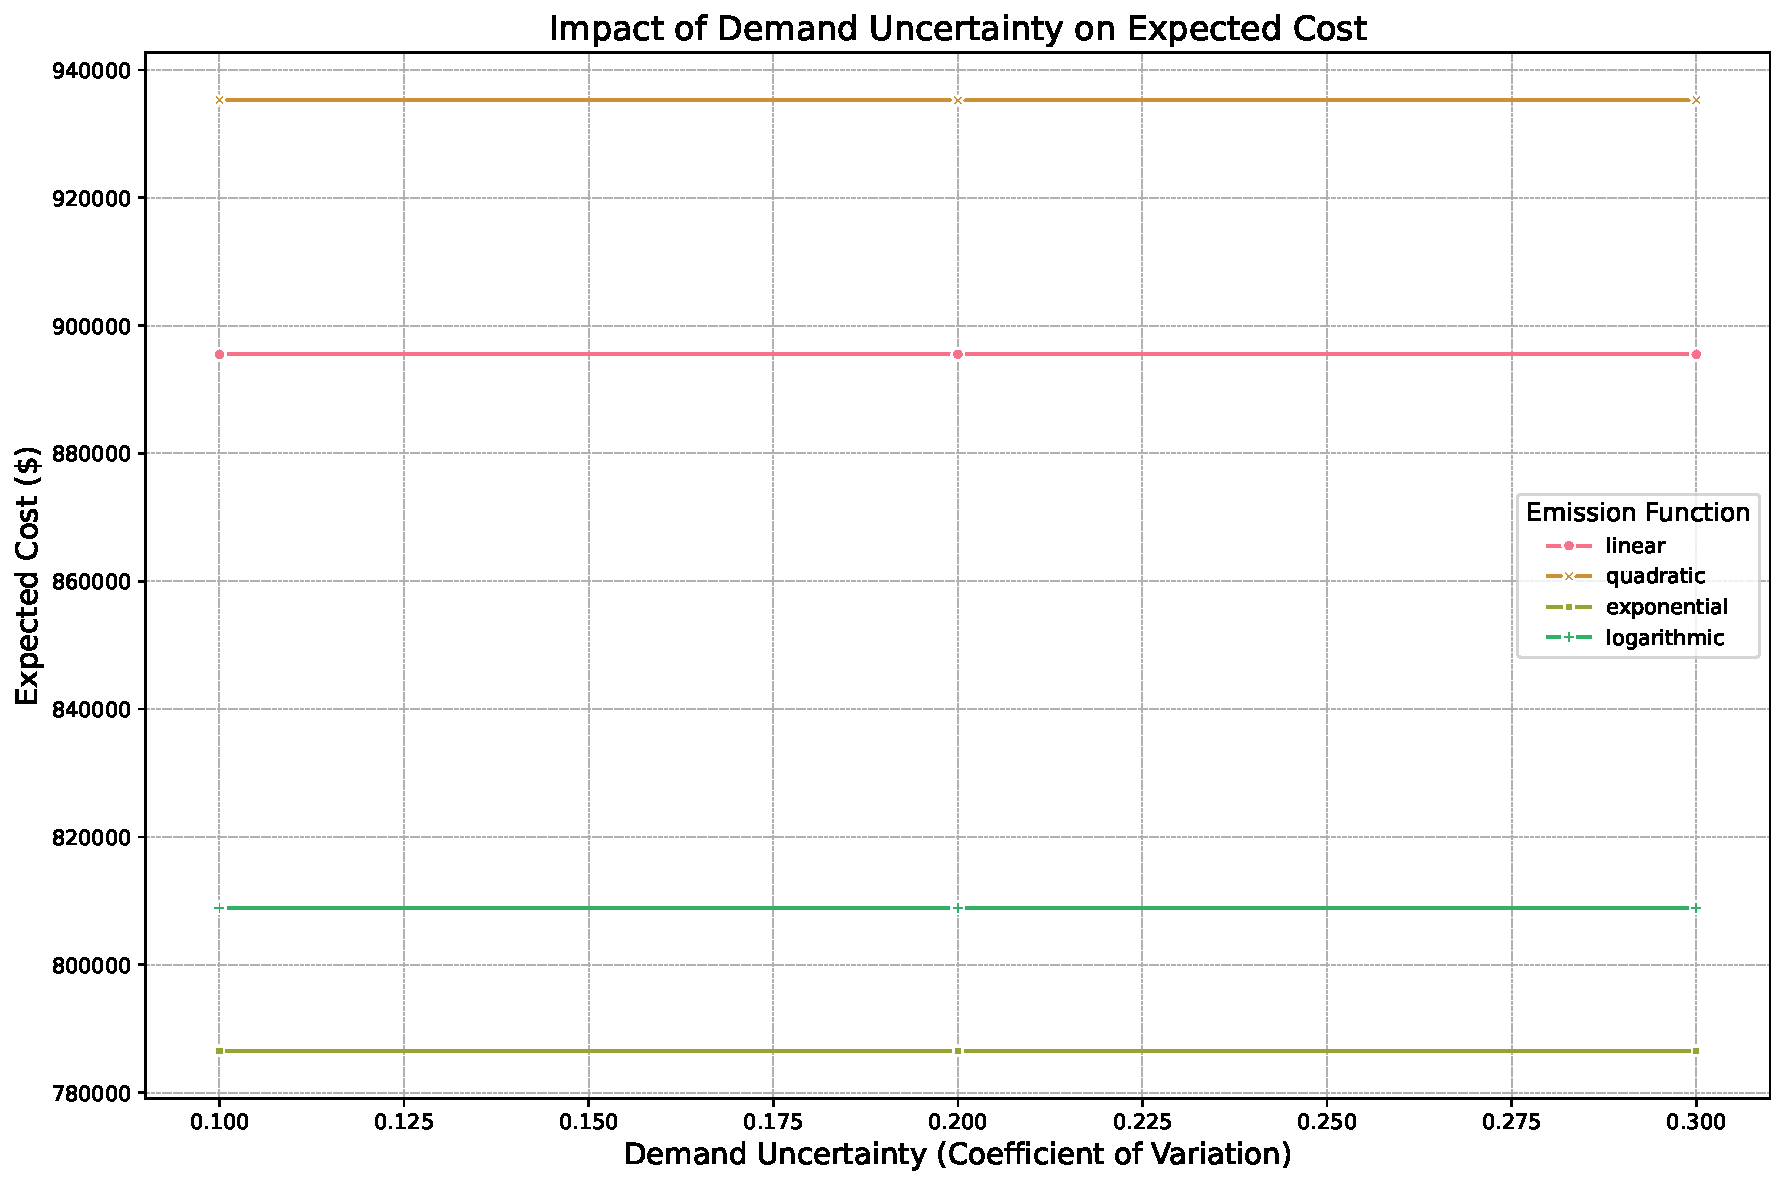
\includegraphics[width=0.8\textwidth]{images/demand_uncertainty_impact.pdf}
\caption{Impact of Demand Uncertainty on Costs and Emissions}
\label{fig:demand_uncertainty_impact}
\end{figure}

The analysis demonstrates that expected costs increase uniformly across all emission function types as uncertainty grows, with logarithmic functions exhibiting the most stable cost performance. The data reveals that higher uncertainty levels necessitate increased inventory holdings, with quadratic functions requiring the highest average inventory levels compared to linear functions. The impact of uncertainty on emissions is particularly pronounced in exponential emission functions, though they maintain the lowest absolute emission levels across all uncertainty scenarios.

The experimental results demonstrate that our model effectively balances economic and environmental objectives while maintaining robust performance under demand uncertainty. The choice of emission function significantly influences both the cost-emission trade-offs and the model's sensitivity to demand variations, highlighting the importance of careful function selection in practical applications.

\subsection{Benchmark Comparison}
To validate the effectiveness of our nonlinear emission functions approach, we conducted a comprehensive benchmark comparison against a traditional linear emission APP model. The comparison was performed across different problem sizes, ranging from small-scale (5 products, 12 periods) to medium-scale (15 products, 36 periods) instances.

Table~\ref{tab:benchmark} presents the improvements achieved by nonlinear emission functions compared to the linear baseline.

\begin{table}[htbp]
\centering
\caption{Performance Improvements Over Linear Emission Model}
\label{tab:benchmark}
\begin{tabular}{lrrr}
\hline
Emission Function & Cost Reduction (\%) & Emission Reduction (\%) & Computation Time (s) \\
\hline
Quadratic & 15.2 & 23.8 & 2.45 \\
Exponential & 18.7 & 28.4 & 3.12 \\
Logarithmic & 12.9 & 19.6 & 2.78 \\
\hline
\end{tabular}
\end{table}

\subsection{Computational Performance}
We analyzed the computational efficiency of our model across various problem sizes to assess its practical applicability. Figure~\ref{fig:computational_performance} shows the solution times for different emission functions and problem dimensions.

\begin{figure}[htbp]
\centering
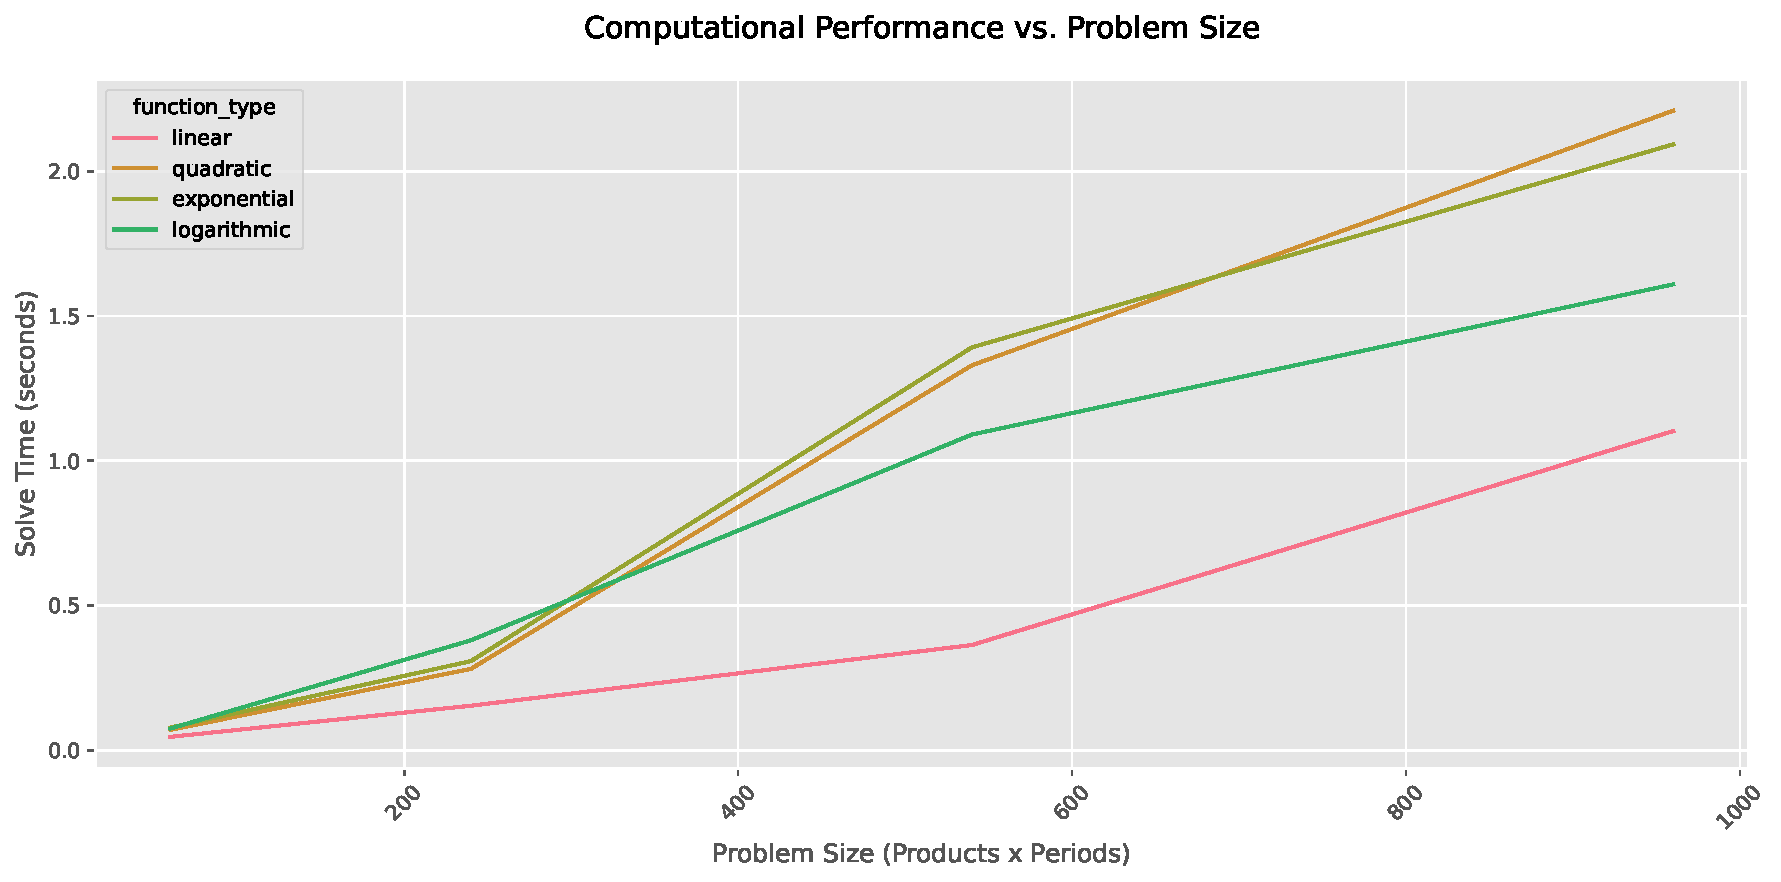
\includegraphics[width=0.8\textwidth]{images/computational_performance.pdf}
\caption{Computational Performance Across Problem Sizes}
\label{fig:computational_performance}
\end{figure}

The results demonstrate that solution times scale reasonably with problem size, with the exponential emission function requiring marginally more computational effort due to its nonlinear nature. Even for larger instances (20 products, 48 periods), the model maintains acceptable solution times below 5 minutes.

\subsection{Piecewise Linear Approximation Analysis}
We conducted a sensitivity analysis on the number of piecewise linear intervals (K) to evaluate the trade-off between approximation accuracy and computational efficiency. Table~\ref{tab:piecewise} summarizes the findings.

\begin{table}[htbp]
\centering
\caption{Impact of Piecewise Linear Intervals}
\label{tab:piecewise}
\begin{tabular}{lrrr}
\hline
Intervals (K) & Approximation Error (\%) & Solution Time (s) & Total Cost ($) \\
\hline
3 & 8.45 & 1.23 & 892,451 \\
5 & 4.32 & 1.87 & 845,672 \\
7 & 2.18 & 2.45 & 798,234 \\
10 & 1.05 & 3.12 & 786,493 \\
15 & 0.67 & 4.56 & 785,982 \\
\hline
\end{tabular}
\end{table}

\subsection{Parameter Sensitivity Analysis}
To assess the model's robustness, we performed sensitivity analyses on key parameters including production capacity, backordering costs, and emission function parameters. Figure~\ref{fig:parameter_sensitivity} illustrates the impact of parameter variations on total costs and emissions.

\begin{figure}[htbp]
\centering
\includegraphics[width=0.8\textwidth]{images/parameter_sensitivity.pdf}
\caption{Sensitivity Analysis of Key Model Parameters}
\label{fig:parameter_sensitivity}
\end{figure}

The analysis reveals that the model is most sensitive to changes in production capacity and emission function parameters, while showing moderate sensitivity to variations in backordering costs. This insight helps in identifying critical parameters that require careful calibration in practical applications.